\section{Process' Perspective}

\subsection{Developer interactions}
The team interacts via Discord and our usual meeting at ITU on tuesdays from 10-18 and extended if needed.

\subsection{Team organization}
We functioned as a cross functional team, sometimes working alone and other times working together typically in pairs. Every opinion/input was acknowledged. 

\subsection{CI/CD chains}
The main three CI/CD chains is

\subsection{Organization of Repository}
The project only consists of a single repository containing the application. This repository contains several folders, 
each containing different files: \\

\begin{table}[]
    \centering
    \begin{tabular}{|l|l|}
    \hline
    \textbf{.github/workflows} & Contains all our workflow files used with Github Actions.                                                                                                          \\ \hline
    \textbf{api\_test}         & Includes files to run the simulator and a test of the API. Primarily used during development of the endpoints.                                                     \\ \hline
    \textbf{remote\_files}     & Has all files that are used when deploying to the server. This includes various logging and monitoring files, our deploy script, and the docker-compose file.      \\ \hline
    \textbf{report}            & This folder is where our report files are saved.                                                                                                                   \\ \hline
    \textbf{src}               & Contains all our application code which is further divided into subfolders, thereby separating the logic of the system.                                            \\ \hline
    \textbf{tests}             & Our test files are located in this folder. It contains a Docker file, docker-compose file, and a test file such that we can run our tests without external impact. \\ \hline
    \end{tabular}
    \caption{Repository folders}
    \label{tab:repo_folders}
    \end{table}

\subsection{Branching strategy}
We used two different branches as a static part of our branching strategy throughout the development of the project. 
The main branch was used as our primary branch on which only functioning and tested code was meant to be pushed. It was
also the code on this branch we used to deploy our application. 

\begin{figure}[H]
    \centering
    \captionsetup{justification=centering,margin=1cm}
    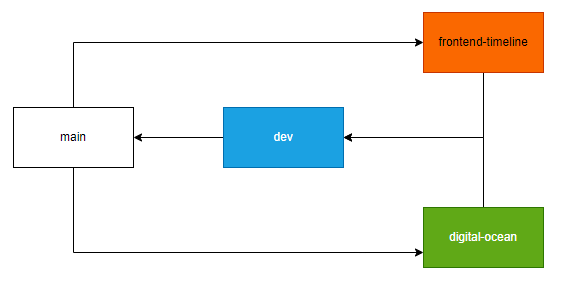
\includegraphics[width=0.8\linewidth]{report/images/branching.png}
    \caption{Branching strategy}
    \label{fig:minitwit}
\end{figure}


\subsection{Development process and tools}
%https://dazzling-screen-208.notion.site/0d2059fc70b34671a8cd3f4f733d4909?v=0b5db8d8c829404e8ae96bb76ca5e6b7



\subsection{Monitoring}

\subsection{Logging}

\subsection{Security assessment}
From our security assessment we worked on blocking the risks with the highest likelihood. The first is \textit{An attacker could gain unauthorized access to the codebase}
- An attacker could easily find passwords and usernames in our public codebase. Now these are in github secrets such that an adversary cannot just 
find these at the public codebase. Another precaution would be to work with the risk \textit{Weak authentication and authorization mechanisms}
 - We are using default values such as postgres as username and password for the database. These should ofc be changed to something following the
 new security protocols standards. 

 \subsection{Scaling and load balancing}

 \subsection{AI-assistants}